\documentclass[multi=tikzpicture,border=8pt]{standalone}
\usepackage[UTF8]{ctex}
\usepackage{amsmath,amssymb,tikz}
\usetikzlibrary{arrows.meta,calc,decorations.pathmorphing}
\definecolor{blue}{HTML}{17365D}
\definecolor{red}{HTML}{AC3931}
\tikzset{every node/.style={font=\small},arrow/.style={-{Stealth[length=2.8mm]},thick},dim/.style={|<->|,thin}}
\begin{document}
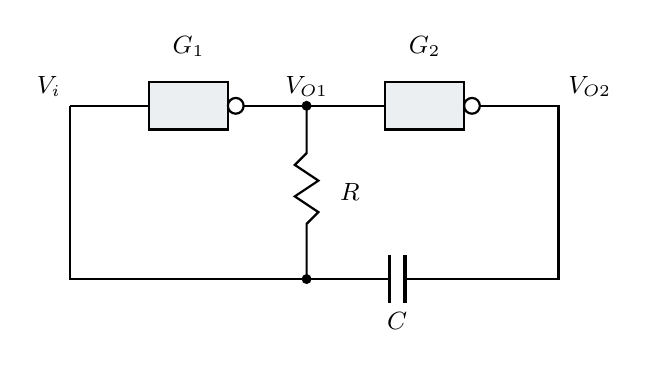
\begin{tikzpicture}

\draw[thick](0,0)--(1,0);\draw[thick,fill=blue!8](1,-.3)rectangle(2,.3);\draw[thick](2.1,0)circle(.1);
\draw[thick](2.2,0)--(4,0);\draw[thick,fill=blue!8](4,-.3)rectangle(5,.3);\draw[thick](5.1,0)circle(.1);\draw[thick](5.2,0)--(6.2,0)--(6.2,-2.2)--(4.25,-2.2);
\draw[very thick](4.25,-2.5)--(4.25,-1.9);\draw[very thick](4.05,-2.5)--(4.05,-1.9);
\draw[thick](4.05,-2.2)--(0,-2.2)--(0,0);
\draw[thick](3,0)--(3,-.6)--(2.85,-.75)--(3.15,-.95)--(2.85,-1.15)--(3.15,-1.35)--(3,-1.5)--(3,-2.2);
\fill(3,0)circle(1.8pt);\fill(3,-2.2)circle(1.8pt);
\node[above]at(1.5,.5){$G_1$};\node[above]at(4.5,.5){$G_2$};
\node[above left]at(0,0){$V_i$};\node[above]at(3,0){$V_{O1}$};\node[above right]at(6.2,0){$V_{O2}$};
\node[right]at(3.3,-1.1){$R$};\node[below]at(4.15,-2.5){$C$};

\end{tikzpicture}
\begin{tikzpicture}

\node[draw,align=center]at(0,1){$V_{O2}=0$\\$V_{O1}=12\,\mathrm V$\\$V_i\to12\,\mathrm V$};
\node[draw,align=center]at(5,1){$V_{O2}=12\,\mathrm V$\\$V_{O1}=0$\\$V_i\to0$};
\draw[arrow,blue](1.8,1.7)--(3.1,1.7)node[above,midway]{$V_i\uparrow6$};
\draw[arrow,red](3.1,.1)--(1.8,.1)node[below,midway]{$V_i\downarrow6$};
\node[below]at(2.5,-1){两个输出始终互补};

\end{tikzpicture}
\begin{tikzpicture}

\node[align=center]at(0,1.4){上升翻转前\\$V_i=6$，$V_{O2}=0$};
\node[align=center]at(5,1.4){上升翻转后\\$V_i=18$，$V_{O2}=12$};
\draw[arrow,blue](1.8,1.4)--(3.2,1.4)node[above,midway]{均增12};
\node[align=center]at(0,-.6){下降翻转前\\$V_i=6$，$V_{O2}=12$};
\node[align=center]at(5,-.6){下降翻转后\\$V_i=-6$，$V_{O2}=0$};
\draw[arrow,red](1.8,-.6)--(3.2,-.6)node[above,midway]{均减12};
\node[below]at(2.5,-1.8){电容电压$u_C=V_i-V_{O2}$连续};

\end{tikzpicture}
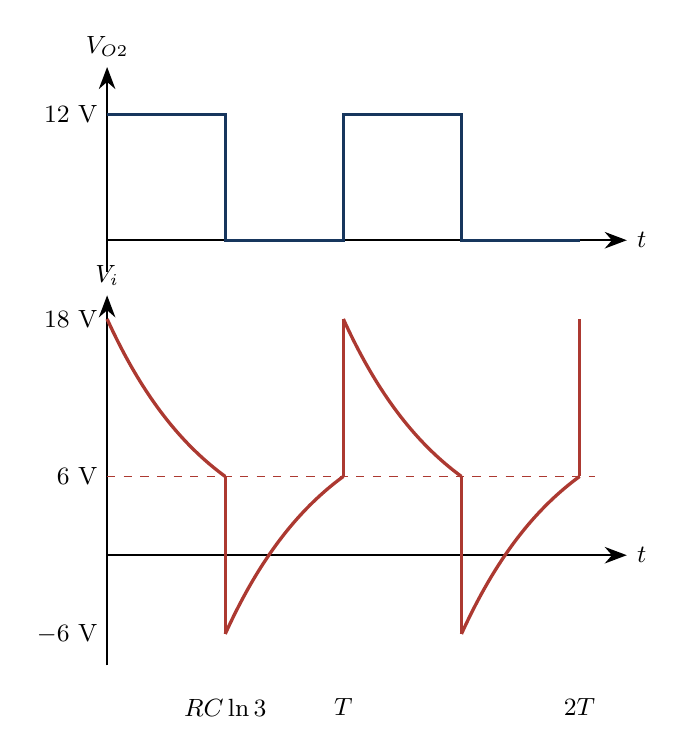
\begin{tikzpicture}
\draw[arrow](0,0)--(6.6,0)node[right]{$t$};\draw[arrow](0,-.4)--(0,2.2)node[above]{$V_{O2}$};\draw[blue,very thick](0,1.6)--(1.5,1.6)--(1.5,0)--(3,0)--(3,1.6)--(4.5,1.6)--(4.5,0)--(6,0);\node[left]at(0,1.6){12 V};\draw[arrow](0,-4)--(6.6,-4)node[right]{$t$};\draw[arrow](0,-5.4)--(0,-.7)node[above]{$V_i$};\draw[dashed,red](0,-3)--(6.2,-3);
\draw[red,very thick]plot coordinates{(0.00000,-1.00000) (0.02344,-1.05106) (0.04688,-1.10125) (0.07031,-1.15058) (0.09375,-1.19908) (0.11719,-1.24675) (0.14062,-1.29361) (0.16406,-1.33967) (0.18750,-1.38494) (0.21094,-1.42945) (0.23437,-1.47320) (0.25781,-1.51620) (0.28125,-1.55848) (0.30469,-1.60003) (0.32812,-1.64087) (0.35156,-1.68103) (0.37500,-1.72049) (0.39844,-1.75929) (0.42187,-1.79742) (0.44531,-1.83491) (0.46875,-1.87176) (0.49219,-1.90798) (0.51562,-1.94358) (0.53906,-1.97858) (0.56250,-2.01299) (0.58594,-2.04680) (0.60938,-2.08005) (0.63281,-2.11272) (0.65625,-2.14484) (0.67969,-2.17642) (0.70312,-2.20745) (0.72656,-2.23796) (0.75000,-2.26795) (0.77344,-2.29743) (0.79688,-2.32640) (0.82031,-2.35489) (0.84375,-2.38289) (0.86719,-2.41041) (0.89062,-2.43746) (0.91406,-2.46406) (0.93750,-2.49020) (0.96094,-2.51589) (0.98437,-2.54115) (1.00781,-2.56598) (1.03125,-2.59039) (1.05469,-2.61438) (1.07812,-2.63796) (1.10156,-2.66114) (1.12500,-2.68393) (1.14844,-2.70632) (1.17188,-2.72834) (1.19531,-2.74998) (1.21875,-2.77126) (1.24219,-2.79217) (1.26562,-2.81273) (1.28906,-2.83293) (1.31250,-2.85280) (1.33594,-2.87232) (1.35938,-2.89151) (1.38281,-2.91038) (1.40625,-2.92892) (1.42969,-2.94715) (1.45312,-2.96507) (1.47656,-2.98269) (1.50000,-3.00000)};
\draw[red,very thick](1.5,-3)--(1.5,-5);
\draw[red,very thick]plot coordinates{(1.50000,-5.00000) (1.52344,-4.94894) (1.54688,-4.89875) (1.57031,-4.84942) (1.59375,-4.80092) (1.61719,-4.75325) (1.64062,-4.70639) (1.66406,-4.66033) (1.68750,-4.61506) (1.71094,-4.57055) (1.73438,-4.52680) (1.75781,-4.48380) (1.78125,-4.44152) (1.80469,-4.39997) (1.82812,-4.35913) (1.85156,-4.31897) (1.87500,-4.27951) (1.89844,-4.24071) (1.92188,-4.20258) (1.94531,-4.16509) (1.96875,-4.12824) (1.99219,-4.09202) (2.01562,-4.05642) (2.03906,-4.02142) (2.06250,-3.98701) (2.08594,-3.95320) (2.10938,-3.91995) (2.13281,-3.88728) (2.15625,-3.85516) (2.17969,-3.82358) (2.20312,-3.79255) (2.22656,-3.76204) (2.25000,-3.73205) (2.27344,-3.70257) (2.29688,-3.67360) (2.32031,-3.64511) (2.34375,-3.61711) (2.36719,-3.58959) (2.39062,-3.56254) (2.41406,-3.53594) (2.43750,-3.50980) (2.46094,-3.48411) (2.48438,-3.45885) (2.50781,-3.43402) (2.53125,-3.40961) (2.55469,-3.38562) (2.57812,-3.36204) (2.60156,-3.33886) (2.62500,-3.31607) (2.64844,-3.29368) (2.67188,-3.27166) (2.69531,-3.25002) (2.71875,-3.22874) (2.74219,-3.20783) (2.76562,-3.18727) (2.78906,-3.16707) (2.81250,-3.14720) (2.83594,-3.12768) (2.85938,-3.10849) (2.88281,-3.08962) (2.90625,-3.07108) (2.92969,-3.05285) (2.95312,-3.03493) (2.97656,-3.01731) (3.00000,-3.00000)};
\draw[red,very thick](3,-3)--(3,-1);
\draw[red,very thick]plot coordinates{(3.00000,-1.00000) (3.02344,-1.05106) (3.04688,-1.10125) (3.07031,-1.15058) (3.09375,-1.19908) (3.11719,-1.24675) (3.14062,-1.29361) (3.16406,-1.33967) (3.18750,-1.38494) (3.21094,-1.42945) (3.23438,-1.47320) (3.25781,-1.51620) (3.28125,-1.55848) (3.30469,-1.60003) (3.32812,-1.64087) (3.35156,-1.68103) (3.37500,-1.72049) (3.39844,-1.75929) (3.42188,-1.79742) (3.44531,-1.83491) (3.46875,-1.87176) (3.49219,-1.90798) (3.51562,-1.94358) (3.53906,-1.97858) (3.56250,-2.01299) (3.58594,-2.04680) (3.60938,-2.08005) (3.63281,-2.11272) (3.65625,-2.14484) (3.67969,-2.17642) (3.70312,-2.20745) (3.72656,-2.23796) (3.75000,-2.26795) (3.77344,-2.29743) (3.79688,-2.32640) (3.82031,-2.35489) (3.84375,-2.38289) (3.86719,-2.41041) (3.89062,-2.43746) (3.91406,-2.46406) (3.93750,-2.49020) (3.96094,-2.51589) (3.98438,-2.54115) (4.00781,-2.56598) (4.03125,-2.59039) (4.05469,-2.61438) (4.07812,-2.63796) (4.10156,-2.66114) (4.12500,-2.68393) (4.14844,-2.70632) (4.17188,-2.72834) (4.19531,-2.74998) (4.21875,-2.77126) (4.24219,-2.79217) (4.26562,-2.81273) (4.28906,-2.83293) (4.31250,-2.85280) (4.33594,-2.87232) (4.35938,-2.89151) (4.38281,-2.91038) (4.40625,-2.92892) (4.42969,-2.94715) (4.45312,-2.96507) (4.47656,-2.98269) (4.50000,-3.00000)};
\draw[red,very thick](4.5,-3)--(4.5,-5);
\draw[red,very thick]plot coordinates{(4.50000,-5.00000) (4.52344,-4.94894) (4.54688,-4.89875) (4.57031,-4.84942) (4.59375,-4.80092) (4.61719,-4.75325) (4.64062,-4.70639) (4.66406,-4.66033) (4.68750,-4.61506) (4.71094,-4.57055) (4.73438,-4.52680) (4.75781,-4.48380) (4.78125,-4.44152) (4.80469,-4.39997) (4.82812,-4.35913) (4.85156,-4.31897) (4.87500,-4.27951) (4.89844,-4.24071) (4.92188,-4.20258) (4.94531,-4.16509) (4.96875,-4.12824) (4.99219,-4.09202) (5.01562,-4.05642) (5.03906,-4.02142) (5.06250,-3.98701) (5.08594,-3.95320) (5.10938,-3.91995) (5.13281,-3.88728) (5.15625,-3.85516) (5.17969,-3.82358) (5.20312,-3.79255) (5.22656,-3.76204) (5.25000,-3.73205) (5.27344,-3.70257) (5.29688,-3.67360) (5.32031,-3.64511) (5.34375,-3.61711) (5.36719,-3.58959) (5.39062,-3.56254) (5.41406,-3.53594) (5.43750,-3.50980) (5.46094,-3.48411) (5.48438,-3.45885) (5.50781,-3.43402) (5.53125,-3.40961) (5.55469,-3.38562) (5.57812,-3.36204) (5.60156,-3.33886) (5.62500,-3.31607) (5.64844,-3.29368) (5.67188,-3.27166) (5.69531,-3.25002) (5.71875,-3.22874) (5.74219,-3.20783) (5.76562,-3.18727) (5.78906,-3.16707) (5.81250,-3.14720) (5.83594,-3.12768) (5.85938,-3.10849) (5.88281,-3.08962) (5.90625,-3.07108) (5.92969,-3.05285) (5.95312,-3.03493) (5.97656,-3.01731) (6.00000,-3.00000)};
\draw[red,very thick](6,-3)--(6,-1);\node[left]at(0,-1){18 V};\node[left]at(0,-3){6 V};\node[left]at(0,-5){$-6$ V};\node[below]at(1.5,-5.7){$RC\ln3$};\node[below]at(3,-5.7){$T$};\node[below]at(6,-5.7){$2T$};
\end{tikzpicture}
\begin{tikzpicture}

\draw[arrow](0,0)--(6.2,0)node[right]{$t/(RC)$};\draw[arrow](0,0)--(0,3)node[above]{$V_i$};
\draw[blue,very thick,domain=0:.693147,samples=50]plot({\x*3},{2*(1-exp(-\x))});
\draw[blue,very thick](2.07944,1)--(2.07944,3);
\draw[blue,very thick,domain=.693147:1.791759,samples=70]plot({\x*3},{3*exp(-\x+.693147)});
\draw[red,dashed](0,1)--(5.8,1)node[right]{6 V};
\node[left]at(0,3){18 V};\node[below]at(2.07944,-.1){$\ln2$};\node[below]at(5.37528,-.1){$\ln2+\ln3$};
\node[above]at(2.8,3.5){无初始电荷且选择第二输出为0};

\end{tikzpicture}
\end{document}
